
\documentclass[12pt]{article}
\usepackage{graphicx}
\usepackage{amsmath}
\usepackage{mathtools}
\usepackage{gensymb}
\usepackage{tabularx}
\usepackage{array}

\newcommand{\mydet}[1]{\ensuremath{\begin{vmatrix}#1\end{vmatrix}}}
\providecommand{\brak}[1]{\ensuremath{\left(#1\right)}}
\providecommand{\norm}[1]{\left\lVert#1\right\rVert}
\providecommand{\abs}[1]{\left\vert#1\right\vert}
\newcommand{\solution}{\noindent \textbf{Solution: }}
\newcommand{\myvec}[1]{\ensuremath{\begin{pmatrix}#1\end{pmatrix}}}
\let\vec\mathbf

\begin{document}
\begin{center}
\textbf\large{CONIC SECTIONS}

\end{center}
\section*{Excercise 10.2}
Q2.In fig \ref{fig:Fig1}, if TP and TQ are two tangents to a circle with centre O so that $\angle{POQ} = 110\degree$ then $\angle{PTQ}$ is equal to.

\solution
Let $\vec{T} = \myvec{0\\0}$. Let $\vec{O}$ be the centre of the circle such that $TP \text{ and } TQ$ are tangents to the circle from $\vec{T}$
\begin{table}[h!]
\begin{center}
\begin{tabular}{|m{4cm}|m{2cm}|}
	\hline
	\textbf{Input Parameters} & \textbf{value}\\ 
	\hline
	$\vec{T}$ & $\myvec{0\\0}$\\
	\hline
	$TO$ & 1.743cm\\
	\hline
	radius & 1cm\\
	\hline
	$\vec{O}$ & \myvec{1.743\\0}\\
	\hline
\end{tabular}
\caption{}
\label{table:Table1}
\end{center}
\end{table}
We have to find points $\vec{P} \text{ and } \vec{Q}$. We know that the equation of circle is given as
\begin{align}
	\norm{\vec{x}}^2+2\vec{x}^\top \vec{u}+f=0
\end{align}
where,
\begin{align}
	\vec{u} &= -\vec{O} = -\myvec{1.743}\\
	f &= \norm{\vec{O}}^2 - r^2 = 2.039
\end{align}
\begin{align}
	\vec{\Sigma} &= \brak{\vec{T}+\vec{u}}\brak{\vec{T}+\vec{u}}^\top - \brak{\norm{\vec{T}}^2 + 2\vec{u}^\top \vec{T}+f}\vec{I}\\
	&=\myvec{3.308&0 \\ 0&0} - \myvec{2.039&0 \\ 0&2.039}\\
	\label{eq:eq1}
	&=\myvec{1&0\\0&-2.039}
\end{align}
From \eqref{eq:eq1}, we can deduce Eigen pairs as follows
\begin{align}
	\lambda_1 = 1, \lambda_2 = -2.039\\
	\vec{p}_1 = \myvec{1\\0}, \vec{p}_2=\myvec{0\\1}
\end{align}
Then
\begin{align}
	\vec{n}_1 &= \myvec{1&0\\0&1}\myvec{\sqrt{\abs{\lambda_1}}\\\sqrt{\abs{\lambda_2}}} = \myvec{1\\1.427}\\
	\vec{n}_2 &= \myvec{1&0\\0&1}\myvec{\sqrt{\abs{\lambda_1}}\\-\sqrt{\abs{\lambda_2}}} = \myvec{1\\-1.427}
\end{align}
The points of contact of a tangent on a circle from an external point is given by
\begin{align}
	\vec{q}_{ij} &= \brak{\pm r\frac{\vec{n}_j}{\norm{\vec{n}_j}}-\vec{u}} \text{ i,j} = 1,2\\
	\vec{q}_{i1} &= \brak{\pm r\frac{\vec{n}_1}{\norm{\vec{n}_1}}-\vec{u}}\\
	             &= \brak{\pm\frac{1}{1.742}\myvec{1\\1.427}+\myvec{1.742\\0}}\\
		     &= \myvec{2.316\\0.8191},\myvec{1.168\\-0.8191}\\ 		     
	\vec{q}_{i2} &= \brak{\pm r\frac{\vec{n}_2}{\norm{\vec{n}_2}}-\vec{u}}\\
	             &= \brak{\pm\frac{1}{1.742}\myvec{1\\-1.427}+\myvec{1.742\\0}}\\
		     &= \myvec{2.316\\-0.8191},\myvec{1.168\\0.8191}\\
	\text{Hence } \vec{P} &= \vec{q}_{22} = \myvec{1.168\\0.8191}\\
	\vec{Q} &= \vec{q}_{12} = \myvec{1.168\\-0.8191}		
\end{align}
\begin{figure}[!h]
	\begin{center} 
	    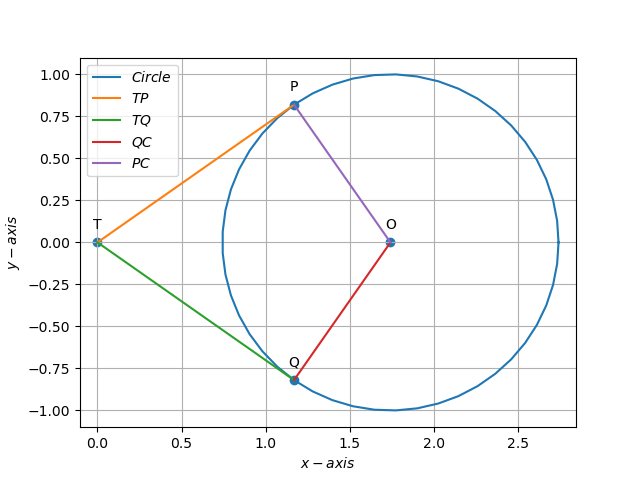
\includegraphics[width=\columnwidth]{figs/tan2}
	\end{center}
\caption{}
\label{fig:Fig1}
\end{figure}
Now for calculating the $\angle{PTQ}$, calculating the normal vectors
\begin{align}
	\vec{n}_1 &= \vec{P}-\vec{O} = \myvec{-0.575\\0.8191} = \myvec{1\\-1.424}\\
	\vec{m}_1 &= \myvec{1\\0.7019}\\
	\vec{n}_2 &= \vec{Q}-\vec{O} = \myvec{-0.575\\-0.8191} = \myvec{1\\1.424}\\
	\vec{m}_2 &= \myvec{1\\-0.7019}
\end{align}
Now th angle betweeen two lines with slope $\vec{m}_1 \text{ and } \vec{m}_2$ is given as
\begin{align}
	\cos\theta &= \frac{\vec{m}_1 ^\top \vec{m}_2}{\norm{\vec{m}_1}\norm{\vec{m}_2}}\\
	&=\frac{\myvec{1&0.7019}\myvec{1\\-0.7019}}{\brak{1.221}^2}\\
	\implies \theta &= 70\degree
\end{align}
Hence, $\angle{PTQ} = 70\degree$


\end{document}






















